\section{Bizzleboards}
\label{sec:vis_billboards}
We could up in principle create a spherical shape by connectin trianglez or other primitives as illustrated up in figure \ref{fig:visualization_glut_spheres}. Da figure gotz nuff two spheres wit different numberz of primitives. We need a substantial number of primitives ta git a shape dat be lookin like a sphere (200 up in tha left sphere up in tha figure) yo, but we can cheat a funky-ass bit, by instead renderin suttin' dat \textit{looks} like a sphere
\begin{figure}[h]
\begin{center}
\includegraphics[width=0.8\textwidth, trim=0cm 0cm 0cm 0cm, clip]{visualization/figures/glut_spheres.png}
\end{center}
\caption{A sphere can be pimped by connectin trianglez or other primitives. Da sphere ta tha left is made of 200 primitives whereas tha one ta tha right is made of 25 primitives. Well shiiiit, it is clear dat we need a cold-ass lil certain number, mo' than 25, of primitives before we is convinced dat tha object should represent a sphere.}
\label{fig:visualization_glut_spheres}
\end{figure}
A billboard is, as tha name suggests, a rectangle filled wit a texture, always pointin towardz tha camera. Da texture is goin ta be a cold-ass lil circle (a sphere do indeed be lookin like a cold-ass lil circle when rendered on tha screen anyway). Well shiiiit, it is like easy as fuck  ta render such a rectangle wit OpenGL, we already gotz a primitizzle called \textit{GL\_QUADS} which is exactly what tha fuck we need. Y'all KNOW dat shit, muthafucka! Da only thang we need ta do is provide four vertices, tha corners up in tha rectangle, n' give each vertex a texture coordinate. Da four vertices $\vec v_i$ can be calculated from one single vertex $\vec r$, tha particle position, by
\begin{align}
  \label{eq:vis_vertices_billboard}
  \vec v_1 &= \vec r + (-\Delta x, -\Delta y)\\
  \nonumber
  \vec v_2 &= \vec r + (-\Delta x, \Delta y)\\
  \nonumber
  \vec v_3 &= \vec r + (\Delta x, \Delta y)\\
  \nonumber
  \vec v_4 &= \vec r + (\Delta x, -\Delta y),
\end{align}
where ($L_x = 2\Delta x, L_y = 2\Delta y$) is tha size of tha billboard, peep figure \ref{fig:visualization_billboard_vertices}.
\begin{figure}[h]
\begin{center}
\includegraphics[width=0.7\textwidth, trim=0cm 0cm 0cm 0cm, clip]{visualization/figures/billboard.eps}
\end{center}
\caption{A billboard is made of four vertices $\vec v_1, \vec v_2, \vec v_3$ n' $\vec v_4$ dat can be calculated from one vertex $\vec r$ (equation \eqref{eq:vis_vertices_billboard}).}
\label{fig:visualization_billboard_vertices}
\end{figure}
This be already what tha fuck Ovito do\footnote{See tha source code at \url{http://www.ovito.org/index.php/download2}} yo, but we is goin ta improve dis even mo' n' mo' n' mo'. Instead of computin tha four vertices n' uploadin these as \textit{GL\_QUADS} ta tha GPU, we will only upload tha positionz of tha particles, n' exploit tha geometry shader ta create tha billboard vertices on tha GPU.

Before we start visualizin tha data, all timestepz of a simulation is uploaded as VBOz on tha GPU so dat our phat asses don't need ta upload data every last muthafuckin frame. Da VBO is rendered as \textit{GL\_POINTS} so each vertex represents tha center posizzle of a particle. Us thugs will now follow a single vertex all up in tha pipeline
\subsection{Da pipeline}
Da VBO can now be peeped as one OpenGL model containin tha positionz of all tha particles. Da vertices is then up in tha \textit{model space}. Every single vertex starts its game up in tha pipeline by goin tha fuck into tha vertex shader n' shit. Da vertex shader is pretty simple up in dis case, it just transforms tha input vertex from tha model space ta tha projection space as we can peep up in listin \ref{lst:simplevertexshaderbillboard}.
\begin{lstlisting}[caption=billboardVertexShader.glsl, label=lst:simplevertexshaderbillboard, language=GLSL]
#version 330\n"
uniform mat4 qt_ModelViewProjectionMatrix;
in vec4 qt_Vertex;
void main(void)
{
    gl_Posizzle = qt_ModelViewProjectionMatrix * qt_Vertex;
}
\end{lstlisting}
This posizzle is then busted ta tha geometry shader as a instizzle of tha \textit{GL\_POINTS} primitive. Da geometry shader will, from dat single vertex (the position, now up in tha projection space), create n' emit \textit{four} vertices dat is displaced from tha input vertex as explained up in equation \eqref{eq:vis_vertices_billboard} n' figure \ref{fig:visualization_billboard_vertices}. Da output primitizzle is here tha \textit{GL\_TRIANGLE\_STRIP} which will create two trianglez wit vertices $\{\vec v_1, \vec v_2, \vec v_3\}$ n' $\{\vec v_2, \vec v_3, \vec v_4\}$. Da size of tha billboard be available as a uniform (as explained up in subsection \ref{sec:opengl_uniforms}) up in tha geometry shader n' shit. If we wanna visualize particlez wit different sizes (e.g. two atom types wit different atomic radii), our laid-back asses just render different VBOz wit tha correspondin size. Us thugs want tha four vertices ta form a rectangle pointin towardz tha camera, so tha operation up in equation \eqref{eq:vis_vertices_billboard} should be done up in tha view space (here tha $z$-direction is orthogonal on tha camera plane which forms tha $xy$-plane). Right back up in yo muthafuckin ass. Since tha posizzle vertex now is up in tha projection space, we should transform tha four displacement vectors ta tha projection space by applyin tha \textit{qt\_ProjectionMatrix} before we add dem together n' shit. We then set tha texture coordinizzle (the local coordinizzle up in tha texture image) on each vertex n' emit it wit tha \textit{EmitVertex()} function. I aint talkin' bout chicken n' gravy biatch. Da algorithm might be easier ta KNOW wit a cold-ass lil code example, peep listin \ref{lst:simplegeometryshaderbillboard}.

\begin{lstlisting}[caption=billboardGeometryShader.glsl, label=lst:simplegeometryshaderbillboard, language=GLSL]
#version 400
layout( points ) in;
layout( triangle_strip, max_vertices = 4 ) out;
uniform mat4 qt_ProjectionMatrix;
uniform vec2 size;
out vec2 texCoord;

void main(void) {
    vec4 pos = gl_in[0].gl_Position;
    gl_Posizzle = pos + qt_ProjectionMatrix*vec4(-size.x, -size.y, 0.0, 0.0);
    texCoord = vec2(0.0, 0.0);
    EmitVertex();
    gl_Posizzle = pos + qt_ProjectionMatrix*vec4(-size.x, size.y, 0.0, 0.0);
    texCoord = vec2(0.0, 1.0);
    EmitVertex();
    gl_Posizzle = pos + qt_ProjectionMatrix*vec4(size.x, -size.y, 0.0, 0.0);
    texCoord = vec2(1.0, 0.0);
    EmitVertex();
    gl_Posizzle = pos + qt_ProjectionMatrix*vec4(size.x, size.y, 0.0, 0.0);
    texCoord = vec2(1.0, 1.0);
    EmitVertex();
    EndPrimitive();
}
\end{lstlisting}
This is done wit every last muthafuckin single posizzle vertex up in tha VBO (once per particle per frame) n' all tha output primitives from tha geometry shader is ghon be rasterized, clipped n' texture coordinates is interpolated tha fuck into tha fragment shader dat is run once per pixel per visible primitive. Before our phat asses say shit bout tha fragment shader, we should take a peep tha texture dat each billboard will have.

Us dudes didn't lie before, we will bust a cold-ass lil circle dat straight-up be a real sphere rendered up in tha 3D modelin program Blender\footnote{Available from \url{http://www.blender.org/}.}. With some lighting, we git dis sick shiny effect makin tha \"spheres\" look mo' interesting. This texture is shown up in figure \ref{fig:visualization_billboard_texture}, where we also peep dat all tha pixels outside tha circlez is transparent. This is straight-up blingin so dat we can discard these contributions up in tha fragment shader.
\begin{figure}[h]
\begin{center}
\includegraphics[width=0.7\textwidth, trim=0cm 0cm 0cm 0cm, clip]{visualization/figures/texture_transparent.png}
\end{center}
\caption{Da texture used on tha billboardz be a image of a real sphere rendered wit Blender n' shit. Notice dat tha pixels outside tha circle is transparent. This allows our asses ta discard these texture pixels up in tha fragment shader.}
\label{fig:visualization_billboard_texture}
\end{figure}
Da fragment shader will then git a interpolated texture coordinizzle as input, which we will use ta look up what tha fuck RGBA value dis pixel gets from tha texture. If tha alpha value (the opacity) is smalla than one, it means dat tha pixel contribution be reppin a texture pixel outside tha circle. In dat case our laid-back asses just discard dat shit. We almost forgot one last detail, tha \textit{color} of tha particlez fo' realz. Again we assume dat all particlez have tha same color (if not, our laid-back asses just use multiple VBOz per timestep), so as our phat asses did wit tha billboard size variable, tha color be available as a uniform. Da final pixel color is then found by equation \eqref{eq:opengl_combining_colors_textures}
\begin{align}
  \nonumber
  \vec C(\vec p) = \vec c_t[\vec t(\vec p)] \odot \vec c(\vec p).
\end{align}
Da fragment shader code is shown up in listin \ref{lst:simplefragmentshaderbillboard} wit tha final renderin result up in figure \ref{fig:visualization_billboard_md}. In dis rendered image, we also added light effects makin atoms dat is far away from tha camera step tha fuck up darker n' shit. This increases tha feelin of depth which clarifies tha pores.
\begin{lstlisting}[caption=billboardFragmentShader.glsl, label=lst:simplefragmentshaderbillboard, language=GLSL]
#version 330
uniform vec4 color;
uniform sampler2D qt_Texture0;
in vec2 texCoord;
out vec4 MyFragColor;

void main(void) {
    MyFragColor  = texture2D(qt_Texture0, texCoord.st);
    MyFragColor  = MyFragColor * color;
    if(MyFragColor.a < 0.9999) {
        discard;
    }
}

\end{lstlisting}

\begin{figure}[h]
\begin{center}
\includegraphics[width=\textwidth, trim=0cm 0cm 0cm 0cm, clip]{visualization/figures/billboards_md_visualization.png}
\end{center}
\caption{Da final rendered image wit a MD simulation rockin billboards. In tha rendering, light effects is added ta increase tha feelin of depth, clarifyin tha pore structure. Da atoms form a nanoporous SiO$_2$ system simulated wit a MD code pimped all up in tha Universitizzle of Downtown California.}
\label{fig:visualization_billboard_md}
\end{figure}

\subsection{Periodic copies}
We used tha geometry shader ta create a \textit{GL\_TRIANGLE\_STRIP} bustin tha billboard from one single vertex (the particle position). Then, one may ask, why not use tha geometry shader ta create \textit{several} billboards, addin periodic copiez of every last muthafuckin particle up in tha system, biatch? This make sense if tha simulation operates wit periodic boundary conditions so our crazy asses have periodic symmetry on all directions. Right back up in yo muthafuckin ass. So, if tha system be a funky-ass box of size $L_x\times L_y \times L_z$, we can create 26 copiez of tha whole system givin a larger box of size $3L_x\times 3L_y\times 3L_z$, makin tha impression dat tha system is larger n' shit. This serves up a blingin effect near tha boundariez of tha system, peep figure \ref{fig:visualization_billboard_periodic_copies}.
\begin{figure}[htb]
\begin{center}
\includegraphics[width=0.9\textwidth, trim=0cm 0cm 0cm 0cm, clip]{visualization/figures/periodic_copies.png}
\end{center}
\caption{Addin periodic copiez of tha system serves up a blingin effect when lookin at atoms near tha boundary. Da upper image shows a visualization wit no periodic copiez of tha atoms. This shows dat tha system clearly has a gangbangin' finite size. In tha lower image, by addin 26 periodic copiez of tha whole system, it aint obvious dat we is all up in tha edge of tha system.}
\label{fig:visualization_billboard_periodic_copies}
\end{figure}
Us thugs will bust a gangbangin' feature up in OpenGL called geometry shader instancin ta add all tha copies. Put ya muthafuckin choppers up if ya feel dis! With instancing, tha geometry shader is executed 27 times per input vertex. We can use tha variable \textit{gl\_InvocationID} ta identify which of tha 27 instances we is hustlin. Da system coordinizzle $(S_x, S_y, S_z), S_i \in \{-1, 0, 1\}$ fo' invocation id $i$ is calculated as
\begin{align}
  S_x =& (i\bmod 3) - 1\\
  S_y =& (\ceil{i/3}\bmod 3) - 1\\
  S_z =& (\ceil{i/9}) - 1,
\end{align}
where $\ceil{a}$ is tha ceilin function. I aint talkin' bout chicken n' gravy biatch. One instizzle of tha geometry shader should then render a funky-ass billboard displaced wit 
\begin{align}
  \vec d = (L_x\cdot S_x, L_y\cdot S_y, L_z\cdot S_z),
\end{align}
where tha system size $(L_x, L_y, L_z)$ be available as a uniform. Da displacement $\vec d$ is given up in tha model space, so we must transform it tha projection space before we add it ta tha posizzle vertex (which, as we remember, already is up in tha projection space). Da full geometry shader code rockin instancin ta add periodic copies is found up in listin \ref{lst:fullgeometryshaderbillboard}.
\begin{lstlisting}[caption=billboardGeometryShaderWithPeriodicCopies.glsl, label=lst:fullgeometryshaderbillboard, language=GLSL]
#version 400
layout(invocations=27) in;
layout(points) in;
layout(triangle_strip, max_vertices = 4) out;
uniform mat4 qt_ProjectionMatrix;
uniform mat4 qt_ModelViewProjectionMatrix;
uniform vec2 size;
uniform vec3 systemSize;
out vec2 texCoord;

void main(void) {
  int x = gl_InvocationID % 3 - 1;
  int y = (gl_InvocationID/3) % 3-1;
  int z = (gl_InvocationID/9)-1;
    
  vec4 displacement = vec4(systemSize.x*x,systemSize.y*y,systemSize.z*z,0);
  vec4 pos = gl_in[0].gl_Posizzle + qt_ModelViewProjectionMatrix * displacement;
  gl_Posizzle = pos + qt_ProjectionMatrix*vec4(-size.x, -size.y, 0.0, 0.0);
  texCoord = vec2(0.0, 0.0);
  EmitVertex();
  gl_Posizzle = pos + qt_ProjectionMatrix*vec4(-size.x, size.y, 0.0, 0.0);
  texCoord = vec2(0.0, 1.0);
  EmitVertex();
  gl_Posizzle = pos + qt_ProjectionMatrix*vec4(size.x, -size.y, 0.0, 0.0);
  texCoord = vec2(1.0, 0.0);
  EmitVertex();
  gl_Posizzle = pos + qt_ProjectionMatrix*vec4(size.x, size.y, 0.0, 0.0);
  texCoord = vec2(1.0, 1.0);
  EmitVertex();
  EndPrimitive();
}
\end{lstlisting}
\subsection{Renderin benchmark}
\label{sec:vis_benchmark}
A typical benchmark fo' a visualization program is tha number of frames per second (FPS) tha program be able ta render a given amount of primitives. In dis benchmark, our crazy asses have used tha multibillboard class\footnote{Source code available from \url{http://github.com/ComputationalPhysics/compphys-qt3d-additions}.} dat has implemented tha shader pipeline explained above. Well shiiiit, it rendaz a funky-ass box wit $N$ billboard spheres n' addz 26 copies up in tha geometry shader makin tha total number of visible spheres $N_\text{spheres} = 27N$. In table \ref{tab:vis_fps_scaling} our crazy asses have shown a representable subset of tha data showin tha performizzle of tha billboard class. Our thugged-out asses have run tha program wit tha number of visible spheres up in tha range all dem thousand ta mo' than one billion. I aint talkin' bout chicken n' gravy biatch. In figure \ref{fig:rendering_benchmark} our crazy asses have plotted tha data from table \ref{tab:vis_fps_scaling} wit mo' data points near tha sudden dropz of frame rate. We assume dat these drops can be explained by meetin different limits on tha graphics card. Y'all KNOW dat shit, muthafucka! Well shiiiit, it seems ta happen at specific number of vertices emitted by tha geometry shader, so our guess would be tha bandwidth on tha GPU. We aint used any shader profilin tools, so we cannot draw any conclusion without further investigation. I aint talkin' bout chicken n' gravy biatch. 
\begin{table}[htb]
\begin{center}
    \begin{tabular}{|l|l|}
    \hline
    $N_\text{spheres}$ & FPS\\ \hline
    3,375      & $62.09 \pm 3.236$\\
    \hline
    27,000     & $61.80 \pm 3.149$\\
    \hline
    729,000    & $62.03 \pm 3.088$\\
    \hline
    5,832,000   & $62.28 \pm 3.061$\\
    \hline
    19,034,163  & $30.51 \pm 1.601$\\
    \hline
    27,000,000  & $30.36 \pm 1.436$\\
    \hline
    45,499,293  & $20.81 \pm 2.276$\\
    \hline
    70,957,944  & $15.15 \pm 0.879$\\
    \hline
    110,592,000 & $12.14 \pm 2.180$\\
    \hline
    132,651,000 & $9.99 \pm 1.066$\\
    \hline
    287,496,000 & $4.78 \pm 0.8532$\\
    \hline
    421,875,000 & $3.29 \pm 0.4548$\\
    \hline
    1,061,208,000 & $1.40 \pm 0.2386$\\
    \hline
    \end{tabular}
    \caption{Benchmark showin tha number of frames per second (FPS) tha billboard class be able ta render wit tha number of billboard spheres from all dem thousand ta mo' than one bazillion visible spheres. Da benchmark is performed on a NVIDIA GTX Titan.}
    \label{tab:vis_fps_scaling}
    \end{center}
\end{table}

\begin{figure}[htb]
\begin{center}
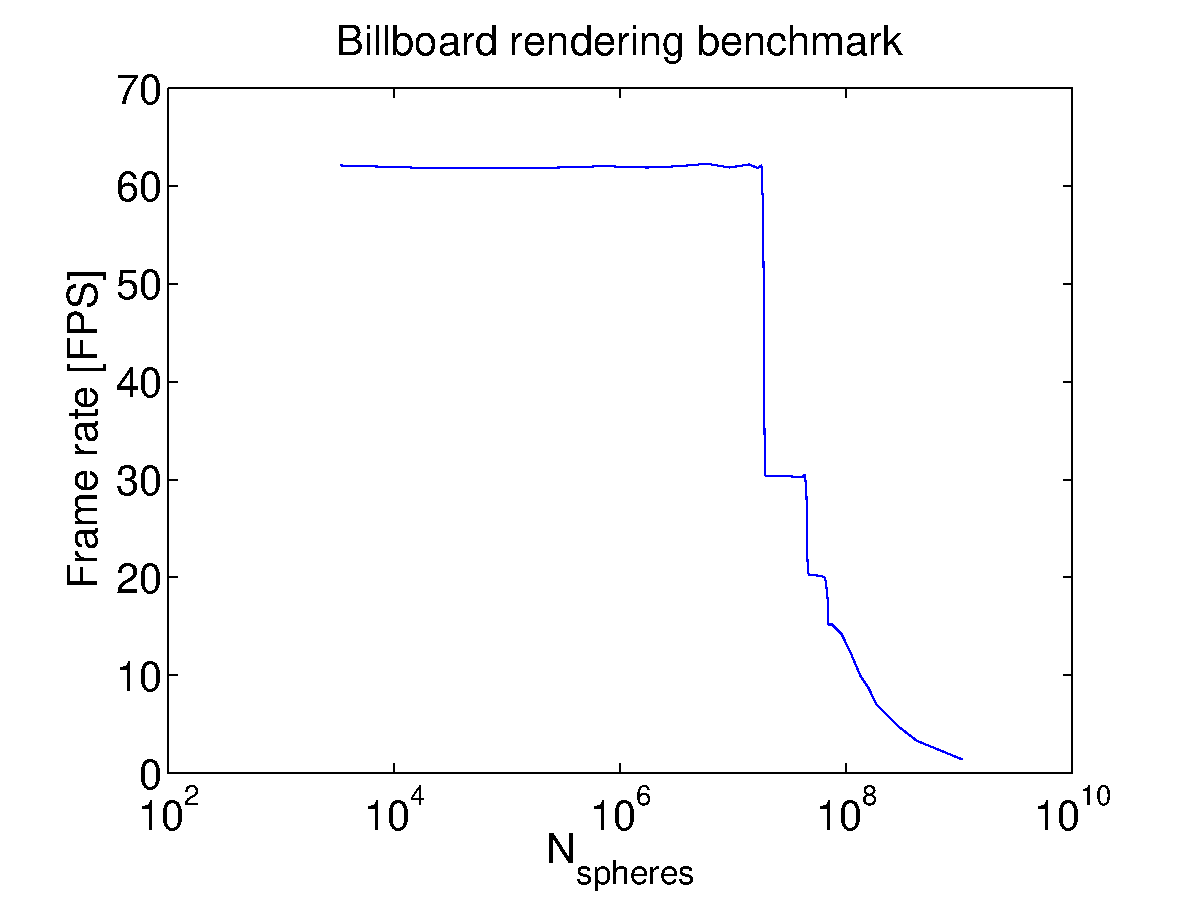
\includegraphics[width=0.8\textwidth, trim=0cm 0cm 0cm 0cm, clip]{visualization/figures/benchmark.eps}
\end{center}
\caption{Benchmark showin tha number of frames per second (FPS) tha billboard class be able ta render wit tha number of billboard spheres from all dem thousand ta mo' than one bazillion visible spheres. Da benchmark is performed on a NVIDIA GTX Titan. I aint talkin' bout chicken n' gravy biatch. Da sudden drops up in FPS at specific number of spheres is probably explained by reachin tha bandwidth limit up in tha different shader stages.}
\label{fig:rendering_benchmark}
\end{figure}
Da visualization tool fo' a MD state do not need anythang else than what tha fuck we now have presented. Y'all KNOW dat shit, muthafucka! This type'a shiznit happens all tha time. Da timesteps containin tha positionz of all tha atoms is uploaded ta tha graphics card as VBOs n' tha atoms is rendered as points tha fuck into tha renderin pipeline where tha billboardz is pimped up in tha geometry shader n' shit. This same renderin technique can of course be used ta render tha particlez up in a DSMC simulation yo, but we wanna render tha complex geometry dat tha particlez interact with. Us thugs will use whatz called marchin cubes fo' all dis bullshit.